\section*{Zadanie 3.}
\begin{task}
Narysować obwiednię pól $E$, $H$, $B$, jaka powstanie w wyniku padania fali o częstotliwości $0.5\ GHz$ rozchodzącej się w kierunku $+Ox$ w układzie trzech ośrodków:\\
I $\hspace{1cm}$ $\epsilon=2\epsilon_{0} \hspace{1cm} \mu=\mu_{0} \hspace{1cm} \sigma=0 \hspace{4cm}$ dla $x<0$\\
II $\hspace{0.86cm}$ $\epsilon=2\epsilon_{0} \hspace{0.97cm} \mu=2\mu_{0} \hspace{0.85cm} \sigma=0 \hspace{4cm}$ dla $0\le x<a$\\
III $\hspace{0.73cm}$ $\epsilon=\epsilon_{0} \hspace{1.15cm} \mu=4\mu_{0} \hspace{0.84cm} \sigma=0 \hspace{4cm}$ dla $a\le x$\\
Przy a=15cm. W każdą obwiednię wpisać kilka krzywych obrazujących chwilowe rozkłady pola.\\
\textbf{Uwaga:} Zwrócić uwagę na możliwość zmiany długości fali przy przekraczaniu granicy ośrodków.\\
\end{task}

\begin{solution}

$$Z_{1}=Z_{0}\sqrt{\cfrac{\mu_{r}}{\epsilon_{r}}}=60\sqrt{2}\pi \ \ \ Z_{2}=Z_{0}\sqrt{\cfrac{2}{2}}=120\pi\ \ \ \ Z_{3}=Z_{0}\sqrt{\cfrac{4}{1}}=240\pi$$\\
$\beta_{2}=\cfrac{20}{3}\pi \ \ \implies \ \lambda_{2}=0.3m=2d \ \implies$ w 2. ośrodku mieści się dokładnie pół długości fali, więc: $Z_{in}=Z_{3}$
$$\Gamma_{1,2}=\cfrac{Z_{in}-Z_{1}}{Z_{in}+Z_{1}}\approx\cfrac{1}{2} \ \ \ \ \Gamma_{2,3}=\cfrac{Z_{3}-Z_{2}}{Z_{3}+Z_{2}}=\cfrac{1}{3}$$

$$WFS_{1}=\cfrac{1+|\Gamma_{1,2}|}{1-|\Gamma_{1,2}|}=3 \ \ \ \ WFS_{2}=\cfrac{1+|\Gamma_{2,3}|}{1-|\Gamma_{2,3}|}=2$$ 

$$E_{1max}=\Gamma_{1,2}E_{0}+E_{0}=\cfrac{3}{2}E_{0} \ \ \ \ E_{1min}=\cfrac{E_{1max}}{WFS_{1}}=\cfrac{1}{2} \ \ \ \ E_{2max}=E_{1max} \ \ \ E_{2min}=\cfrac{E_{2max}}{WFS_{2}}=\cfrac{3}{4}E_{0}$$

\begin{center}
$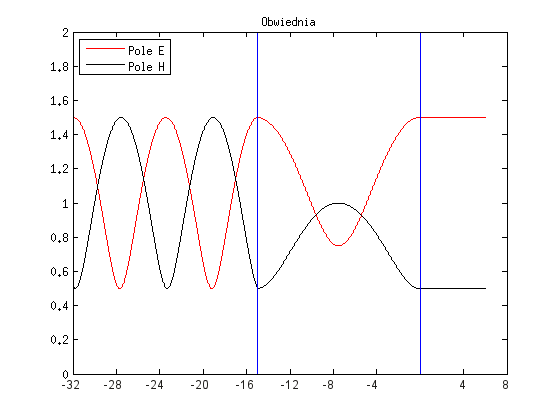
\includegraphics[scale=1]{3_1}$\\
\end{center}
\begin{center}
$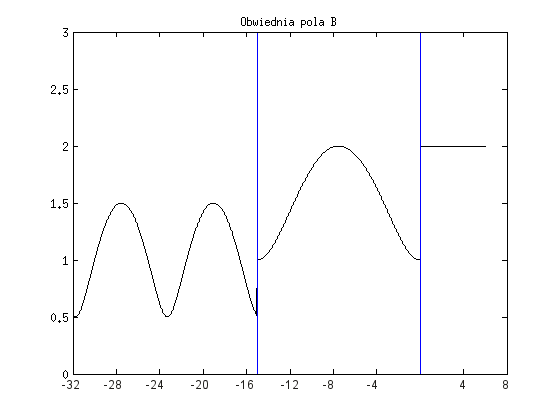
\includegraphics[scale=1]{3_2}$\\
\end{center}

\end{solution}